% Options for packages loaded elsewhere
\PassOptionsToPackage{unicode}{hyperref}
\PassOptionsToPackage{hyphens}{url}
\PassOptionsToPackage{dvipsnames,svgnames,x11names}{xcolor}
%
\documentclass[
  a4paperpaper,
]{article}

\usepackage{amsmath,amssymb}
\usepackage{iftex}
\ifPDFTeX
  \usepackage[T1]{fontenc}
  \usepackage[utf8]{inputenc}
  \usepackage{textcomp} % provide euro and other symbols
\else % if luatex or xetex
  \ifXeTeX
    \usepackage{mathspec} % this also loads fontspec
  \else
    \usepackage{unicode-math} % this also loads fontspec
  \fi
  \defaultfontfeatures{Scale=MatchLowercase}
  \defaultfontfeatures[\rmfamily]{Ligatures=TeX,Scale=1}
\fi
\usepackage{lmodern}
\ifPDFTeX\else  
    % xetex/luatex font selection
\fi
% Use upquote if available, for straight quotes in verbatim environments
\IfFileExists{upquote.sty}{\usepackage{upquote}}{}
\IfFileExists{microtype.sty}{% use microtype if available
  \usepackage[]{microtype}
  \UseMicrotypeSet[protrusion]{basicmath} % disable protrusion for tt fonts
}{}
\makeatletter
\@ifundefined{KOMAClassName}{% if non-KOMA class
  \IfFileExists{parskip.sty}{%
    \usepackage{parskip}
  }{% else
    \setlength{\parindent}{0pt}
    \setlength{\parskip}{6pt plus 2pt minus 1pt}}
}{% if KOMA class
  \KOMAoptions{parskip=half}}
\makeatother
\usepackage{xcolor}
\setlength{\emergencystretch}{3em} % prevent overfull lines
\setcounter{secnumdepth}{-\maxdimen} % remove section numbering
% Make \paragraph and \subparagraph free-standing
\ifx\paragraph\undefined\else
  \let\oldparagraph\paragraph
  \renewcommand{\paragraph}[1]{\oldparagraph{#1}\mbox{}}
\fi
\ifx\subparagraph\undefined\else
  \let\oldsubparagraph\subparagraph
  \renewcommand{\subparagraph}[1]{\oldsubparagraph{#1}\mbox{}}
\fi

\usepackage{color}
\usepackage{fancyvrb}
\newcommand{\VerbBar}{|}
\newcommand{\VERB}{\Verb[commandchars=\\\{\}]}
\DefineVerbatimEnvironment{Highlighting}{Verbatim}{commandchars=\\\{\}}
% Add ',fontsize=\small' for more characters per line
\usepackage{framed}
\definecolor{shadecolor}{RGB}{241,243,245}
\newenvironment{Shaded}{\begin{snugshade}}{\end{snugshade}}
\newcommand{\AlertTok}[1]{\textcolor[rgb]{0.68,0.00,0.00}{#1}}
\newcommand{\AnnotationTok}[1]{\textcolor[rgb]{0.37,0.37,0.37}{#1}}
\newcommand{\AttributeTok}[1]{\textcolor[rgb]{0.40,0.45,0.13}{#1}}
\newcommand{\BaseNTok}[1]{\textcolor[rgb]{0.68,0.00,0.00}{#1}}
\newcommand{\BuiltInTok}[1]{\textcolor[rgb]{0.00,0.23,0.31}{#1}}
\newcommand{\CharTok}[1]{\textcolor[rgb]{0.13,0.47,0.30}{#1}}
\newcommand{\CommentTok}[1]{\textcolor[rgb]{0.37,0.37,0.37}{#1}}
\newcommand{\CommentVarTok}[1]{\textcolor[rgb]{0.37,0.37,0.37}{\textit{#1}}}
\newcommand{\ConstantTok}[1]{\textcolor[rgb]{0.56,0.35,0.01}{#1}}
\newcommand{\ControlFlowTok}[1]{\textcolor[rgb]{0.00,0.23,0.31}{#1}}
\newcommand{\DataTypeTok}[1]{\textcolor[rgb]{0.68,0.00,0.00}{#1}}
\newcommand{\DecValTok}[1]{\textcolor[rgb]{0.68,0.00,0.00}{#1}}
\newcommand{\DocumentationTok}[1]{\textcolor[rgb]{0.37,0.37,0.37}{\textit{#1}}}
\newcommand{\ErrorTok}[1]{\textcolor[rgb]{0.68,0.00,0.00}{#1}}
\newcommand{\ExtensionTok}[1]{\textcolor[rgb]{0.00,0.23,0.31}{#1}}
\newcommand{\FloatTok}[1]{\textcolor[rgb]{0.68,0.00,0.00}{#1}}
\newcommand{\FunctionTok}[1]{\textcolor[rgb]{0.28,0.35,0.67}{#1}}
\newcommand{\ImportTok}[1]{\textcolor[rgb]{0.00,0.46,0.62}{#1}}
\newcommand{\InformationTok}[1]{\textcolor[rgb]{0.37,0.37,0.37}{#1}}
\newcommand{\KeywordTok}[1]{\textcolor[rgb]{0.00,0.23,0.31}{#1}}
\newcommand{\NormalTok}[1]{\textcolor[rgb]{0.00,0.23,0.31}{#1}}
\newcommand{\OperatorTok}[1]{\textcolor[rgb]{0.37,0.37,0.37}{#1}}
\newcommand{\OtherTok}[1]{\textcolor[rgb]{0.00,0.23,0.31}{#1}}
\newcommand{\PreprocessorTok}[1]{\textcolor[rgb]{0.68,0.00,0.00}{#1}}
\newcommand{\RegionMarkerTok}[1]{\textcolor[rgb]{0.00,0.23,0.31}{#1}}
\newcommand{\SpecialCharTok}[1]{\textcolor[rgb]{0.37,0.37,0.37}{#1}}
\newcommand{\SpecialStringTok}[1]{\textcolor[rgb]{0.13,0.47,0.30}{#1}}
\newcommand{\StringTok}[1]{\textcolor[rgb]{0.13,0.47,0.30}{#1}}
\newcommand{\VariableTok}[1]{\textcolor[rgb]{0.07,0.07,0.07}{#1}}
\newcommand{\VerbatimStringTok}[1]{\textcolor[rgb]{0.13,0.47,0.30}{#1}}
\newcommand{\WarningTok}[1]{\textcolor[rgb]{0.37,0.37,0.37}{\textit{#1}}}

\providecommand{\tightlist}{%
  \setlength{\itemsep}{0pt}\setlength{\parskip}{0pt}}\usepackage{longtable,booktabs,array}
\usepackage{calc} % for calculating minipage widths
% Correct order of tables after \paragraph or \subparagraph
\usepackage{etoolbox}
\makeatletter
\patchcmd\longtable{\par}{\if@noskipsec\mbox{}\fi\par}{}{}
\makeatother
% Allow footnotes in longtable head/foot
\IfFileExists{footnotehyper.sty}{\usepackage{footnotehyper}}{\usepackage{footnote}}
\makesavenoteenv{longtable}
\usepackage{graphicx}
\makeatletter
\def\maxwidth{\ifdim\Gin@nat@width>\linewidth\linewidth\else\Gin@nat@width\fi}
\def\maxheight{\ifdim\Gin@nat@height>\textheight\textheight\else\Gin@nat@height\fi}
\makeatother
% Scale images if necessary, so that they will not overflow the page
% margins by default, and it is still possible to overwrite the defaults
% using explicit options in \includegraphics[width, height, ...]{}
\setkeys{Gin}{width=\maxwidth,height=\maxheight,keepaspectratio}
% Set default figure placement to htbp
\makeatletter
\def\fps@figure{htbp}
\makeatother
% definitions for citeproc citations
\NewDocumentCommand\citeproctext{}{}
\NewDocumentCommand\citeproc{mm}{%
  \begingroup\def\citeproctext{#2}\cite{#1}\endgroup}
\makeatletter
 % allow citations to break across lines
 \let\@cite@ofmt\@firstofone
 % avoid brackets around text for \cite:
 \def\@biblabel#1{}
 \def\@cite#1#2{{#1\if@tempswa , #2\fi}}
\makeatother
\newlength{\cslhangindent}
\setlength{\cslhangindent}{1.5em}
\newlength{\csllabelwidth}
\setlength{\csllabelwidth}{3em}
\newenvironment{CSLReferences}[2] % #1 hanging-indent, #2 entry-spacing
 {\begin{list}{}{%
  \setlength{\itemindent}{0pt}
  \setlength{\leftmargin}{0pt}
  \setlength{\parsep}{0pt}
  % turn on hanging indent if param 1 is 1
  \ifodd #1
   \setlength{\leftmargin}{\cslhangindent}
   \setlength{\itemindent}{-1\cslhangindent}
  \fi
  % set entry spacing
  \setlength{\itemsep}{#2\baselineskip}}}
 {\end{list}}
\usepackage{calc}
\newcommand{\CSLBlock}[1]{\hfill\break\parbox[t]{\linewidth}{\strut\ignorespaces#1\strut}}
\newcommand{\CSLLeftMargin}[1]{\parbox[t]{\csllabelwidth}{\strut#1\strut}}
\newcommand{\CSLRightInline}[1]{\parbox[t]{\linewidth - \csllabelwidth}{\strut#1\strut}}
\newcommand{\CSLIndent}[1]{\hspace{\cslhangindent}#1}

\usepackage{fvextra}
\usepackage[auth-lg]{authblk}
\DefineVerbatimEnvironment{Highlighting}{Verbatim}{breaklines,commandchars=\\\{\}}
\DefineVerbatimEnvironment{OutputCode}{Verbatim}{breaklines,commandchars=\\\{\}}
\makeatletter
\@ifpackageloaded{caption}{}{\usepackage{caption}}
\AtBeginDocument{%
\ifdefined\contentsname
  \renewcommand*\contentsname{Índice}
\else
  \newcommand\contentsname{Índice}
\fi
\ifdefined\listfigurename
  \renewcommand*\listfigurename{Lista de Figuras}
\else
  \newcommand\listfigurename{Lista de Figuras}
\fi
\ifdefined\listtablename
  \renewcommand*\listtablename{Lista de Tabelas}
\else
  \newcommand\listtablename{Lista de Tabelas}
\fi
\ifdefined\figurename
  \renewcommand*\figurename{Figura}
\else
  \newcommand\figurename{Figura}
\fi
\ifdefined\tablename
  \renewcommand*\tablename{Tabela}
\else
  \newcommand\tablename{Tabela}
\fi
}
\@ifpackageloaded{float}{}{\usepackage{float}}
\floatstyle{ruled}
\@ifundefined{c@chapter}{\newfloat{codelisting}{h}{lop}}{\newfloat{codelisting}{h}{lop}[chapter]}
\floatname{codelisting}{Listagem}
\newcommand*\listoflistings{\listof{codelisting}{Lista de Listagens}}
\makeatother
\makeatletter
\makeatother
\makeatletter
\@ifpackageloaded{caption}{}{\usepackage{caption}}
\@ifpackageloaded{subcaption}{}{\usepackage{subcaption}}
\makeatother
\ifLuaTeX
\usepackage[bidi=basic]{babel}
\else
\usepackage[bidi=default]{babel}
\fi
\babelprovide[main,import]{portuguese}
% get rid of language-specific shorthands (see #6817):
\let\LanguageShortHands\languageshorthands
\def\languageshorthands#1{}
\ifLuaTeX
  \usepackage{selnolig}  % disable illegal ligatures
\fi
\usepackage{bookmark}

\IfFileExists{xurl.sty}{\usepackage{xurl}}{} % add URL line breaks if available
\urlstyle{same} % disable monospaced font for URLs
\hypersetup{
  pdftitle={Lista 2},
  pdfauthor={César A. Galvão - 190011572; Gabriela Carneiro - 180120816; João Vitor Vasconcelos - 170126064},
  pdflang={pt},
  colorlinks=true,
  linkcolor={blue},
  filecolor={Maroon},
  citecolor={Blue},
  urlcolor={Blue},
  pdfcreator={LaTeX via pandoc}}

\title{Lista 2}
\author{César A. Galvão - 190011572 \and Gabriela Carneiro -
180120816 \and João Vitor Vasconcelos - 170126064}
\date{}

\begin{document}
\maketitle

\renewcommand*\contentsname{Índice}
{
\hypersetup{linkcolor=}
\setcounter{tocdepth}{2}
\tableofcontents
}
\newpage{}

\section{Questão 3}\label{questuxe3o-3}

Considerando duas classes com distribuição normal multivariada tal que
\(\omega_1 \sim N_2(\boldsymbol{\mu}, \boldsymbol{\Sigma})\) com

\[
\boldsymbol{\mu} = \begin{bmatrix} 1 \\ 0 \end{bmatrix} \quad \text{e} \quad \boldsymbol{\Sigma} = \begin{bmatrix} 1 & 0 \\ 0 & 1 \end{bmatrix} = \boldsymbol{I}_2
\]

e \(\omega_2 \sim N_2(\boldsymbol{\mu}, \boldsymbol{\Sigma})\) com

\[
\boldsymbol{\mu} = \begin{bmatrix} -1 \\ 0 \end{bmatrix} \quad \text{e} \quad \boldsymbol{\Sigma} = \begin{bmatrix} 1 & 0 \\ 0 & 1 \end{bmatrix} = \boldsymbol{I}_2
\] ~

\subsection{Item a}\label{item-a}

Gere 100 valores para \(\omega_1\) e \(\omega_2\).

\begin{center}\rule{0.5\linewidth}{0.5pt}\end{center}

Os valores para as variáveis serão gerados utilizando o algoritmo de
Cholesky disponibilizado na lista, comentada abaixo para facilitar a
compreensão:

\begin{Shaded}
\begin{Highlighting}[]
\NormalTok{rmvn.cholesky }\OtherTok{\textless{}{-}} \ControlFlowTok{function}\NormalTok{( n , mu , Sigma ) \{}
\NormalTok{  p }\OtherTok{\textless{}{-}} \FunctionTok{length}\NormalTok{(mu) }\CommentTok{\# normal p{-}variada}
\NormalTok{  Q }\OtherTok{\textless{}{-}} \FunctionTok{chol}\NormalTok{(Sigma) }\CommentTok{\# \{base\} cholesky decomposition}
\NormalTok{  Z }\OtherTok{\textless{}{-}} \FunctionTok{matrix}\NormalTok{(}\FunctionTok{rnorm}\NormalTok{(n}\SpecialCharTok{*}\NormalTok{p), }\AttributeTok{nrow=}\NormalTok{n, }\AttributeTok{ncol =}\NormalTok{ p) }\CommentTok{\# matriz nxp \textasciitilde{} N\_p(0,1)}
\NormalTok{  X }\OtherTok{\textless{}{-}}\NormalTok{ Z }\SpecialCharTok{\%*\%}\NormalTok{ Q }\SpecialCharTok{+} \CommentTok{\# matriz nxp \textasciitilde{} N\_p(0,Σ)}
          \FunctionTok{matrix}\NormalTok{(mu, n, p, }\AttributeTok{byrow=}\ConstantTok{TRUE}\NormalTok{) }\CommentTok{\#mu\_1 e mu\_2 em cada linha}
  \FunctionTok{return}\NormalTok{(X)}
\NormalTok{\}}
\end{Highlighting}
\end{Shaded}

~

A seguir, é escolhida uma semente para o gerador de números aleatórios e
são geradas as variáveis. Uma prévia dos dados é exibida em seguida.

\begin{Shaded}
\begin{Highlighting}[]
\FunctionTok{set.seed}\NormalTok{(}\DecValTok{11572}\NormalTok{)}

\NormalTok{n }\OtherTok{\textless{}{-}} \DecValTok{100}

\NormalTok{mu1 }\OtherTok{\textless{}{-}} \FunctionTok{c}\NormalTok{(}\DecValTok{1}\NormalTok{, }\DecValTok{0}\NormalTok{)}
\NormalTok{Sigma1 }\OtherTok{\textless{}{-}} \FunctionTok{diag}\NormalTok{(}\DecValTok{2}\NormalTok{)}
\NormalTok{omega1 }\OtherTok{\textless{}{-}} \FunctionTok{rmvn.cholesky}\NormalTok{(n, mu1, Sigma1)}

\NormalTok{mu2 }\OtherTok{\textless{}{-}} \FunctionTok{c}\NormalTok{(}\SpecialCharTok{{-}}\DecValTok{1}\NormalTok{, }\DecValTok{0}\NormalTok{)}
\NormalTok{Sigma2 }\OtherTok{\textless{}{-}} \FunctionTok{diag}\NormalTok{(}\DecValTok{2}\NormalTok{)}
\NormalTok{omega2 }\OtherTok{\textless{}{-}} \FunctionTok{rmvn.cholesky}\NormalTok{(n, mu2, Sigma2)}
\end{Highlighting}
\end{Shaded}

\begin{table}

\caption{\label{tbl-headomega}Primeiras linhas de \(\omega_1\) e
\(\omega_2\).}

\begin{minipage}{0.50\linewidth}

\begin{longtable}[]{@{}rr@{}}
\toprule\noalign{}
V1 & V2 \\
\midrule\noalign{}
\endhead
\bottomrule\noalign{}
\endlastfoot
0.4528201 & 0.2274710 \\
1.2804296 & 1.3931905 \\
-0.0467663 & -1.2357199 \\
1.7315127 & -3.3383750 \\
0.9339194 & 0.0419395 \\
0.7733280 & 1.6790085 \\
\end{longtable}

\end{minipage}%
%
\begin{minipage}{0.50\linewidth}

\begin{longtable}[]{@{}rr@{}}
\toprule\noalign{}
V1 & V2 \\
\midrule\noalign{}
\endhead
\bottomrule\noalign{}
\endlastfoot
-1.3386455 & -1.6352549 \\
0.3181510 & -1.3237408 \\
-1.4029014 & 0.3951291 \\
-0.2880302 & -0.2085144 \\
-2.2679073 & -0.2438205 \\
-0.4362316 & 0.6367181 \\
\end{longtable}

\end{minipage}%

\end{table}%

~

\subsection{Item b}\label{item-b}

Verifique se os valores gerados seguem distribuição
\(N_2(\boldsymbol{\mu}, \boldsymbol{\Sigma})\). Lembre que neste caso, o
par deve seguir uma distribuição \(\chi^2\) e cada variável deve ter
distribuição Normal.

\begin{center}\rule{0.5\linewidth}{0.5pt}\end{center}

Considerando que cada variável deve seguir uma distribuição Normal
univariada e que, neste caso, as matrizes de covariância são identidades
--- ou seja, as normais bivariadas são compostas por normais univariadas
independentes entre si ---, verificamos a normalidade da distribuição de
cada componente de \(\omega_1\) e \(\omega_2\) utilizando gráficos
quantil-quantil e testes Shapiro-Wilk.

O código a seguir exibe a função montada para gerar os gráficos.

\begin{Shaded}
\begin{Highlighting}[]
\NormalTok{plot\_qq\_mtvn }\OtherTok{\textless{}{-}} \ControlFlowTok{function}\NormalTok{(x, var, i)\{}
\NormalTok{  x }\SpecialCharTok{\%\textgreater{}\%} 
\NormalTok{  as\_tibble }\SpecialCharTok{\%\textgreater{}\%}
  \FunctionTok{ggplot}\NormalTok{(}\FunctionTok{aes}\NormalTok{(}\AttributeTok{sample =}\NormalTok{ \{\{ var \}\})) }\SpecialCharTok{+}
  \FunctionTok{geom\_qq}\NormalTok{(}\AttributeTok{alpha =}\NormalTok{ .}\DecValTok{4}\NormalTok{) }\SpecialCharTok{+}
  \FunctionTok{geom\_qq\_line}\NormalTok{() }\SpecialCharTok{+}
  \FunctionTok{labs}\NormalTok{(}\AttributeTok{x =} \StringTok{"Quantis teóricos"}\NormalTok{, }
       \AttributeTok{y =} \FunctionTok{substitute}\NormalTok{(}\FunctionTok{paste}\NormalTok{(}\StringTok{"Quantis observados {-}"}\NormalTok{, omega[i], }\StringTok{"{-}"}\NormalTok{, var), }
                      \FunctionTok{list}\NormalTok{(}\AttributeTok{var =} \FunctionTok{substitute}\NormalTok{(var),}
                      \AttributeTok{i =} \FunctionTok{substitute}\NormalTok{(i)))) }\SpecialCharTok{+}
  \FunctionTok{theme\_bw}\NormalTok{()}\SpecialCharTok{+}
  \FunctionTok{theme}\NormalTok{(}
    \AttributeTok{axis.text =} \FunctionTok{element\_text}\NormalTok{(}\AttributeTok{size =} \FloatTok{7.5}\NormalTok{),}
    \AttributeTok{axis.title =} \FunctionTok{element\_text}\NormalTok{(}\AttributeTok{size =} \FloatTok{7.5}\NormalTok{)}
\NormalTok{  )}
\NormalTok{\}}
\end{Highlighting}
\end{Shaded}

~

Com os gráficos gerados na Figura~\ref{fig-qqplots} a seguir vemos que a
princípio não há motivos para visualmente rejeitar a normalidade dos
dados. As caudas, como é de se esperar, são ou pouco mais pesadas.

\begin{Shaded}
\begin{Highlighting}[]
\FunctionTok{plot\_grid}\NormalTok{(}\FunctionTok{plot\_qq\_mtvn}\NormalTok{(omega1, V1, }\DecValTok{1}\NormalTok{),}
          \FunctionTok{plot\_qq\_mtvn}\NormalTok{(omega1, V2, }\DecValTok{1}\NormalTok{),}
          \FunctionTok{plot\_qq\_mtvn}\NormalTok{(omega2, V1, }\DecValTok{2}\NormalTok{),}
          \FunctionTok{plot\_qq\_mtvn}\NormalTok{(omega2, V2, }\DecValTok{2}\NormalTok{), }\AttributeTok{nrow =} \DecValTok{2}\NormalTok{)}
\end{Highlighting}
\end{Shaded}

\begin{figure}[H]

\centering{

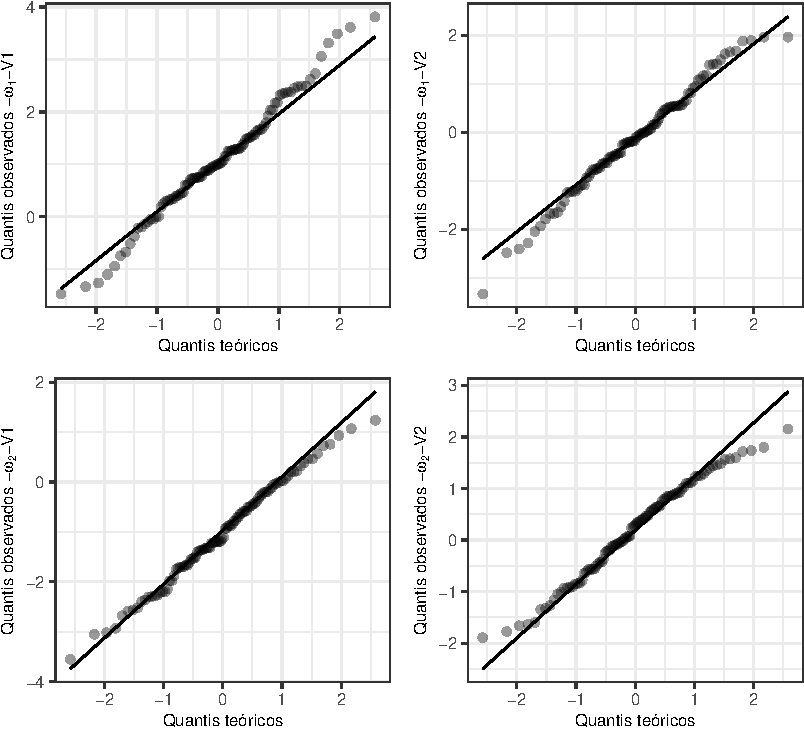
\includegraphics{lista-2_files/figure-pdf/fig-qqplots-1.pdf}

}

\caption{\label{fig-qqplots}QQ-plot para \(\omega_1\) e \(\omega_2\) em
relação à distribuição normal.}

\end{figure}%

\begin{Shaded}
\begin{Highlighting}[]
\FunctionTok{bind\_cols}\NormalTok{(omega1, omega2) }\SpecialCharTok{\%\textgreater{}\%}
  \FunctionTok{as\_tibble}\NormalTok{() }\SpecialCharTok{\%\textgreater{}\%}
  \FunctionTok{summarise}\NormalTok{(}\FunctionTok{across}\NormalTok{(}\FunctionTok{everything}\NormalTok{(), }\SpecialCharTok{\textasciitilde{}} \FunctionTok{shapiro.test}\NormalTok{(.)}\SpecialCharTok{$}\NormalTok{p.value)) }\SpecialCharTok{\%\textgreater{}\%}
\NormalTok{  knitr}\SpecialCharTok{::}\FunctionTok{kable}\NormalTok{(}
    \AttributeTok{col.names =} \FunctionTok{c}\NormalTok{(}\StringTok{"omega1\_V1"}\NormalTok{, }\StringTok{"omega1\_V2"}\NormalTok{, }\StringTok{"omega2\_V1"}\NormalTok{, }\StringTok{"omega2\_V2"}\NormalTok{)}
\NormalTok{  )}
\end{Highlighting}
\end{Shaded}

\begin{longtable}[]{@{}rrrr@{}}

\caption{\label{tbl-testshapiro}Teste de Shapiro-Wilk para componentes
de \(\omega_1\) e \(\omega_2\).}

\tabularnewline

\toprule\noalign{}
omega1\_V1 & omega1\_V2 & omega2\_V1 & omega2\_V2 \\
\midrule\noalign{}
\endhead
\bottomrule\noalign{}
\endlastfoot
0.5506312 & 0.5300882 & 0.8559406 & 0.2021182 \\

\end{longtable}

O teste Henze-Zirkler para normalidade multivariada aponta p-valores
0.58 e 0.29 para \(\omega_1\) e \(\omega_2\), respectivamente, não dando
indícios de que se deva rejeitar a hipótese de normalidade.

Além disso, para uma visualização estilo QQ-plot, utiliza-se
\texttt{heplots::cqplot}. A normalidade multivariada é avaliada
utilizando a distância Malanobis ao quadrado, que conforme Artes e
Barroso (2023), segue a forma:

\begin{align}
  D^2_M = (\boldsymbol{x} - \boldsymbol{\mu})^\top \Sigma^{-1} (\boldsymbol{x} - \boldsymbol{\mu}) \sim \chi^2_p
\end{align}

Na Figura~\ref{fig-qqchisq1} não é possível identificar pontos fora da
banda de confiança, enquanto na Figura~\ref{fig-qqchisq2} é possível ver
alguns pontos de quantis inferiores fora da banda. No entanto, abos os
conjuntos de dados serão considerados normais multivariadas.

\begin{figure}[H]

\centering{

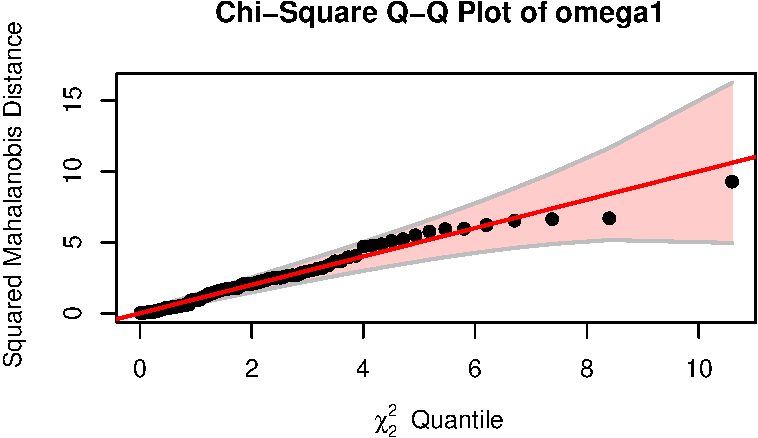
\includegraphics{lista-2_files/figure-pdf/fig-qqchisq1-1.pdf}

}

\caption{\label{fig-qqchisq1}QQ-plot para \(\omega_1\) em relação à
distribuição \(\chi^2\).}

\end{figure}%

\begin{figure}[H]

\centering{

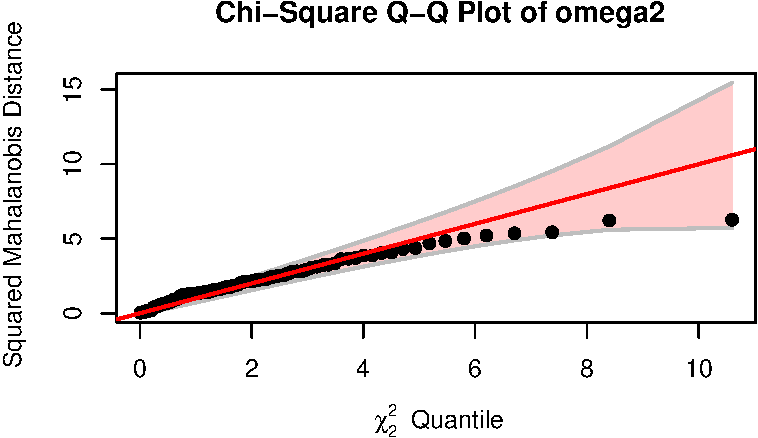
\includegraphics{lista-2_files/figure-pdf/fig-qqchisq2-1.pdf}

}

\caption{\label{fig-qqchisq2}QQ-plot para \(\omega_2\) em relação à
distribuição \(\chi^2\).}

\end{figure}%

\subsection{Item c}\label{item-c}

Para um determinado \(\mu\) na razão de verossimilhança, determine as
regiões \(\Omega_1\) e \(\Omega_2\) na regra de Neyman-Pearson.

\begin{center}\rule{0.5\linewidth}{0.5pt}\end{center}

A seguir é criada uma função para avaliar a razão de verossimilhanças
\(\frac{p(x| \omega_1)}{p(x| \omega_2)}\) para nossos conjuntos de
dados.

\begin{Shaded}
\begin{Highlighting}[]
\NormalTok{p }\OtherTok{=} \DecValTok{2}
\NormalTok{S }\OtherTok{\textless{}{-}} \FunctionTok{diag}\NormalTok{(}\DecValTok{2}\NormalTok{)}

\CommentTok{\# funcao para resolver a exponencial da verossimilhanca}
\NormalTok{expo\_norm }\OtherTok{\textless{}{-}} \ControlFlowTok{function}\NormalTok{(x, mu, S)\{}
\NormalTok{  part1 }\OtherTok{\textless{}{-}} \SpecialCharTok{{-}}\FunctionTok{t}\NormalTok{(}\FunctionTok{t}\NormalTok{(x)}\SpecialCharTok{{-}}\NormalTok{mu) }\SpecialCharTok{\%*\%} \FunctionTok{solve}\NormalTok{(S)}
\NormalTok{  part2 }\OtherTok{\textless{}{-}}\NormalTok{ (x}\SpecialCharTok{{-}}\NormalTok{mu)}
  
  \FunctionTok{return}\NormalTok{(part1[,}\DecValTok{1}\NormalTok{]}\SpecialCharTok{*}\NormalTok{part2[,}\DecValTok{1}\NormalTok{] }\SpecialCharTok{+}\NormalTok{ part1[,}\DecValTok{2}\NormalTok{]}\SpecialCharTok{*}\NormalTok{part2[,}\DecValTok{2}\NormalTok{])}
\NormalTok{\}}

\CommentTok{\#funcao para calcular a razao de verossimilhancas                             }
\NormalTok{razao\_vero }\OtherTok{\textless{}{-}} \ControlFlowTok{function}\NormalTok{(x, p, mu1, mu2, S)\{}
  \FunctionTok{return}\NormalTok{(}
  \CommentTok{\# verossimilhanca sob mu1 dividida por }
   \FunctionTok{exp}\NormalTok{(}\FunctionTok{expo\_norm}\NormalTok{(x, mu1, S)}\SpecialCharTok{/}\DecValTok{2}\NormalTok{)}\SpecialCharTok{/}
    \CommentTok{\# verossimilhanca sob mu2}
   \FunctionTok{exp}\NormalTok{(}\FunctionTok{expo\_norm}\NormalTok{(x, mu2, S)}\SpecialCharTok{/}\DecValTok{2}\NormalTok{)}
\NormalTok{  )}
\NormalTok{\}                             }
\end{Highlighting}
\end{Shaded}

~

Classificaremos considerando as regiões em que a razão de
verossimilhanças dá mais suporte a \(p(x| \omega_1)\) ou
\(p(x| \omega_2)\).

\begin{Shaded}
\begin{Highlighting}[]
\NormalTok{razoes }\OtherTok{\textless{}{-}} \FunctionTok{c}\NormalTok{(}
  \FunctionTok{razao\_vero}\NormalTok{(omega1, }\DecValTok{2}\NormalTok{, mu1, mu2, S),}
  \FunctionTok{razao\_vero}\NormalTok{(omega2, }\DecValTok{2}\NormalTok{, mu1, mu2, S))}
                             
\CommentTok{\# limite da regiao de classificaçao}

\NormalTok{limite }\OtherTok{\textless{}{-}} \FunctionTok{quantile}\NormalTok{(razoes, }\AttributeTok{probs =} \FloatTok{0.5}\NormalTok{)}

\CommentTok{\# tabelas com regioes corretas e classificacao}

\NormalTok{classificacoes }\OtherTok{\textless{}{-}} \FunctionTok{tibble}\NormalTok{(}
  \AttributeTok{regioes\_corretas =} \FunctionTok{rep}\NormalTok{(}\FunctionTok{c}\NormalTok{(}\StringTok{"1"}\NormalTok{, }\StringTok{"2"}\NormalTok{), }\AttributeTok{each =} \DecValTok{100}\NormalTok{),}
  \AttributeTok{x1 =} \FunctionTok{c}\NormalTok{(omega1[,}\DecValTok{1}\NormalTok{], omega2[,}\DecValTok{1}\NormalTok{]),}
  \AttributeTok{x2 =} \FunctionTok{c}\NormalTok{(omega1[,}\DecValTok{2}\NormalTok{], omega2[,}\DecValTok{2}\NormalTok{]),}
  \AttributeTok{razoes =}\NormalTok{ razoes,}
  \AttributeTok{classificacao =} \FunctionTok{if\_else}\NormalTok{(razoes }\SpecialCharTok{\textgreater{}}\NormalTok{ limite, }\StringTok{"1"}\NormalTok{, }\StringTok{"2"}\NormalTok{),}
  \AttributeTok{acertos =} \FunctionTok{if\_else}\NormalTok{(regioes\_corretas }\SpecialCharTok{==}\NormalTok{ classificacao, }\DecValTok{1}\NormalTok{, }\DecValTok{0}\NormalTok{)}
\NormalTok{)}
\end{Highlighting}
\end{Shaded}

~

Quando a razão for superior à mediana das verossimilhanças,
classificaremos como \(\omega_1\) e no complementar quando for inferior
à mediana. Em outras palavras,

\begin{align}
  \boldsymbol{x} \in \Omega_1 \Rightarrow \frac{p(x| \omega_1)}{p(x| \omega_2)} > 1.1583663.
\end{align}

Dessa forma, há 84\% de acertos. A Tabela~\ref{tbl-acertosvero} a seguir
nos dá o desempenho da classificação:

\begin{longtable}[]{@{}lrr@{}}

\caption{\label{tbl-acertosvero}Tabela de contingências de
classificações em \(\omega_1\) e \(\omega_2\) utilizando a regra de
alocação de Neyman-Pearson.}

\tabularnewline

\toprule\noalign{}
& omega1 & omega2 \\
\midrule\noalign{}
\endhead
\bottomrule\noalign{}
\endlastfoot
omega1 & 84 & 16 \\
omega2 & 16 & 84 \\

\end{longtable}

~

Avaliamos graficamente as classificações a seguir:

\begin{Shaded}
\begin{Highlighting}[]
\NormalTok{fig\_corretas }\OtherTok{\textless{}{-}}\NormalTok{ classificacoes }\SpecialCharTok{\%\textgreater{}\%}
  \FunctionTok{ggplot}\NormalTok{(}\FunctionTok{aes}\NormalTok{(}\AttributeTok{x =}\NormalTok{ x1, }\AttributeTok{y =}\NormalTok{ x2, }\AttributeTok{color =}\NormalTok{ regioes\_corretas))}\SpecialCharTok{+}
  \FunctionTok{geom\_point}\NormalTok{()}\SpecialCharTok{+}
  \FunctionTok{theme\_bw}\NormalTok{()}\SpecialCharTok{+}
  \FunctionTok{theme}\NormalTok{(}\AttributeTok{legend.position =} \StringTok{"bottom"}\NormalTok{)}

\NormalTok{fig\_classificadas }\OtherTok{\textless{}{-}}\NormalTok{ classificacoes }\SpecialCharTok{\%\textgreater{}\%}
  \FunctionTok{ggplot}\NormalTok{(}\FunctionTok{aes}\NormalTok{(}\AttributeTok{x =}\NormalTok{ x1, }\AttributeTok{y =}\NormalTok{ x2, }\AttributeTok{color =}\NormalTok{ classificacao))}\SpecialCharTok{+}
  \FunctionTok{geom\_point}\NormalTok{()}\SpecialCharTok{+}
  \FunctionTok{theme\_bw}\NormalTok{()}\SpecialCharTok{+}
  \FunctionTok{theme}\NormalTok{(}\AttributeTok{legend.position =} \StringTok{"bottom"}\NormalTok{)}

\FunctionTok{plot\_grid}\NormalTok{(fig\_corretas, fig\_classificadas)}
\end{Highlighting}
\end{Shaded}

\begin{figure}[H]

\centering{

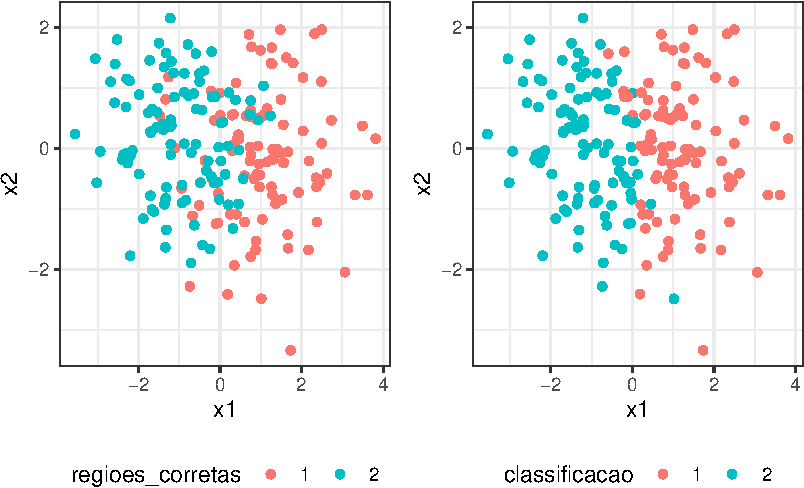
\includegraphics{lista-2_files/figure-pdf/fig-classificacoes-1.pdf}

}

\caption{\label{fig-classificacoes}Grupos reais e preditos nas classes
\(\omega_1\) e \(\omega_2\) utilizando regra de Neyman-Pearson.}

\end{figure}%

~

Este comportamento é esperado, visto que há matrizes de covariância e
\(\mu_2\) iguais, diferindo apenas em \(X_1\).

\subsection{Item d}\label{item-d}

Considere diferentes valores \(\bf{x} = [x_1 , x_2]^\top\) e utilize a
regra de decisão de Bayes para alocar estes valores em \(\Omega_1\) ou
\(\Omega_2\).

\begin{center}\rule{0.5\linewidth}{0.5pt}\end{center}

De acordo com a regra de Bayes,

\begin{align}
  \boldsymbol{x} \in \Omega_1 \Rightarrow \frac{p(x| \omega_1)}{p(x| \omega_2)} > \frac{p(x| \omega_2)}{p(x| \omega_1)}.
\end{align}

Dessa forma, classificamos a seguir as observações:

\begin{Shaded}
\begin{Highlighting}[]
\NormalTok{razoes\_bayes }\OtherTok{\textless{}{-}} \FunctionTok{tibble}\NormalTok{( }\CommentTok{\#monta as razoes de verossimilhanca}
  \AttributeTok{grupos =} \FunctionTok{rep}\NormalTok{(}\FunctionTok{c}\NormalTok{(}\StringTok{"1"}\NormalTok{, }\StringTok{"2"}\NormalTok{), }\AttributeTok{each =} \DecValTok{100}\NormalTok{),}
  \AttributeTok{vero1 =} \FunctionTok{c}\NormalTok{(}\FunctionTok{razao\_vero}\NormalTok{(omega1, }\DecValTok{2}\NormalTok{, mu1, mu2, S), }\FunctionTok{razao\_vero}\NormalTok{(omega2, }\DecValTok{2}\NormalTok{, mu1, mu2, S)),}
  \AttributeTok{vero2 =} \FunctionTok{c}\NormalTok{(}\FunctionTok{razao\_vero}\NormalTok{(omega1, }\DecValTok{2}\NormalTok{, mu2, mu1, S),}\FunctionTok{razao\_vero}\NormalTok{(omega2, }\DecValTok{2}\NormalTok{, mu2, mu1, S)),}
  \AttributeTok{x1 =} \FunctionTok{c}\NormalTok{(omega1[,}\DecValTok{1}\NormalTok{], omega2[,}\DecValTok{1}\NormalTok{]),}
  \AttributeTok{x2 =} \FunctionTok{c}\NormalTok{(omega1[,}\DecValTok{2}\NormalTok{], omega2[,}\DecValTok{2}\NormalTok{])}
\NormalTok{  ) }\SpecialCharTok{\%\textgreater{}\%}
  \FunctionTok{mutate}\NormalTok{(}
    \AttributeTok{classificacao =} \FunctionTok{case\_when}\NormalTok{(}
\NormalTok{      vero1 }\SpecialCharTok{\textgreater{}}\NormalTok{ vero2 }\SpecialCharTok{\textasciitilde{}} \StringTok{"1"}\NormalTok{,}
\NormalTok{      vero2 }\SpecialCharTok{\textgreater{}}\NormalTok{ vero1 }\SpecialCharTok{\textasciitilde{}} \StringTok{"2"}
\NormalTok{    ),}
    \AttributeTok{acertos =} \FunctionTok{if\_else}\NormalTok{(grupos }\SpecialCharTok{==}\NormalTok{ classificacao, }\DecValTok{1}\NormalTok{, }\DecValTok{0}\NormalTok{)}
\NormalTok{  )}
\end{Highlighting}
\end{Shaded}

Nesse caso há 82\% de acertos. A Tabela~\ref{tbl-acertosverobayes} a
seguir nos dá o desempenho da classificação:

\begin{longtable}[]{@{}lrr@{}}

\caption{\label{tbl-acertosverobayes}Tabela de contingências de
classificações em \(\omega_1\) e \(\omega_2\) utilizando regra de
Bayes.}

\tabularnewline

\toprule\noalign{}
& omega1 & omega2 \\
\midrule\noalign{}
\endhead
\bottomrule\noalign{}
\endlastfoot
omega1 & 84 & 16 \\
omega2 & 16 & 84 \\

\end{longtable}

~

Avaliamos graficamente as classificações a seguir:

\begin{Shaded}
\begin{Highlighting}[]
\NormalTok{fig\_corretas\_bayes }\OtherTok{\textless{}{-}}\NormalTok{ razoes\_bayes }\SpecialCharTok{\%\textgreater{}\%}
  \FunctionTok{ggplot}\NormalTok{(}\FunctionTok{aes}\NormalTok{(}\AttributeTok{x =}\NormalTok{ x1, }\AttributeTok{y =}\NormalTok{ x2, }\AttributeTok{color =}\NormalTok{ grupos))}\SpecialCharTok{+}
  \FunctionTok{geom\_point}\NormalTok{()}\SpecialCharTok{+}
  \FunctionTok{theme\_bw}\NormalTok{()}\SpecialCharTok{+}
  \FunctionTok{theme}\NormalTok{(}\AttributeTok{legend.position =} \StringTok{"bottom"}\NormalTok{)}

\NormalTok{fig\_classificadas\_bayes }\OtherTok{\textless{}{-}}\NormalTok{ razoes\_bayes }\SpecialCharTok{\%\textgreater{}\%}
  \FunctionTok{ggplot}\NormalTok{(}\FunctionTok{aes}\NormalTok{(}\AttributeTok{x =}\NormalTok{ x1, }\AttributeTok{y =}\NormalTok{ x2, }\AttributeTok{color =}\NormalTok{ classificacao))}\SpecialCharTok{+}
  \FunctionTok{geom\_point}\NormalTok{()}\SpecialCharTok{+}
  \FunctionTok{theme\_bw}\NormalTok{()}\SpecialCharTok{+}
  \FunctionTok{theme}\NormalTok{(}\AttributeTok{legend.position =} \StringTok{"bottom"}\NormalTok{)}

\FunctionTok{plot\_grid}\NormalTok{(fig\_corretas\_bayes, fig\_classificadas\_bayes)}
\end{Highlighting}
\end{Shaded}

\begin{figure}[H]

\centering{

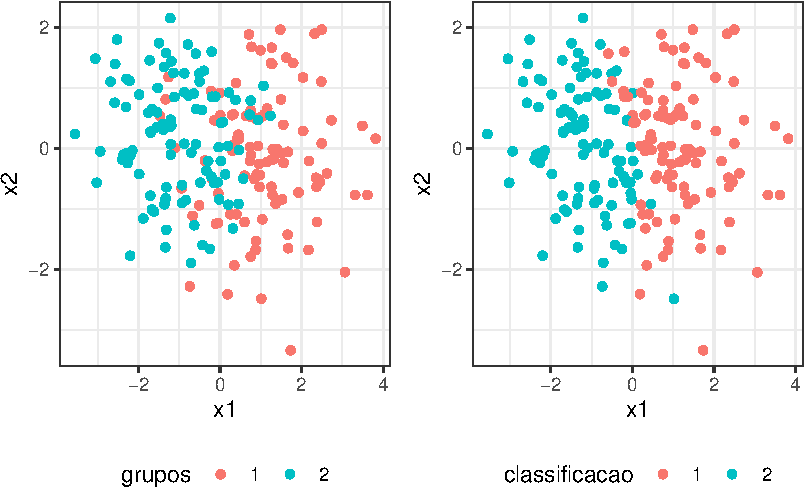
\includegraphics{lista-2_files/figure-pdf/fig-classificacoesbayes-1.pdf}

}

\caption{\label{fig-classificacoesbayes}Grupos reais e preditos nas
classes \(\omega_1\) e \(\omega_2\) utilizando regra de Bayes.}

\end{figure}%

~

Neste caso, utilizando qualquer das regras de classificação se obtém os
mesmos resultados.

\newpage{}

\section{Questão 4}\label{questuxe3o-4}

Considere duas classes com distribuições multivariadas tal que
\(p(x|\omega_1) \sim N_p (\boldsymbol{\mu_1} , \boldsymbol{\Sigma})\) e
\(p(x|\omega_2) \sim N_p (\boldsymbol{\mu_2} , \boldsymbol{\Sigma})\).
Mostre que o logaritmo da razão de verossimilhança é linear em relação
ao vetor de características \(\bf{x}\).

\begin{center}\rule{0.5\linewidth}{0.5pt}\end{center}

Considere a função densidade para a distribuição normal multivariada:

\begin{align}
  f(\boldsymbol{x}) = \frac{1}{(2\pi)^{k/2}|\Sigma|^{1/2}} \exp \{ -\frac{1}{2} (\boldsymbol{x} - \boldsymbol{\mu})^\top \Sigma^{-1} (\boldsymbol{x} - \boldsymbol{\mu}) \}
\end{align}

A razão de verossimilhanças é dada já simplificada em relação às
constantes de normalização por

\begin{align}
  \mathcal{L}(\boldsymbol{x}) &= \frac{p(\boldsymbol{x}|\omega_1)}{p(\boldsymbol{x}|\omega_2)} = \frac{\exp \{ -\frac{1}{2} (\boldsymbol{x} - \boldsymbol{\mu_1})^\top \Sigma^{-1} (\boldsymbol{x} - \boldsymbol{\mu_1}) \}}{\exp \{ -\frac{1}{2} (\boldsymbol{x} - \boldsymbol{\mu_2})^\top \Sigma^{-1} (\boldsymbol{x} - \boldsymbol{\mu_2}) \}} \\
 \ell(\boldsymbol{x}) &=  -\frac{1}{2} (\boldsymbol{x} - \boldsymbol{\mu_1})^\top \Sigma^{-1} (\boldsymbol{x} - \boldsymbol{\mu_1}) + \frac{1}{2} (\boldsymbol{x} - \boldsymbol{\mu_2})^\top \Sigma^{-1} (\boldsymbol{x} - \boldsymbol{\mu_2})\nonumber \\
 &= -\frac{1}{2} \left( \boldsymbol{x}^\top \Sigma^{-1} \boldsymbol{x} - \boldsymbol{x}^\top \Sigma^{-1} \boldsymbol{\mu_1}  - \boldsymbol{\mu_1}^\top \Sigma^{-1} \boldsymbol{x} +  \boldsymbol{\mu_1}^\top \Sigma^{-1} \boldsymbol{\mu_1} \right) \nonumber \\
&+ \frac{1}{2} \left( \boldsymbol{x}^\top \Sigma^{-1} \boldsymbol{x} - \boldsymbol{x}^\top \Sigma^{-1} \boldsymbol{\mu_2}  - \boldsymbol{\mu_2}^\top \Sigma^{-1} \boldsymbol{x} +  \boldsymbol{\mu_2}^\top \Sigma^{-1} \boldsymbol{\mu_2} \right) \nonumber \\
&= \frac{1}{2} \left( \boldsymbol{x}^\top \Sigma^{-1} (\boldsymbol{\mu}_1 - \boldsymbol{\mu}_2) + (\boldsymbol{\mu}_1 - \boldsymbol{\mu}_2)^\top \Sigma^{-1} \boldsymbol{x} + \boldsymbol{\mu_2}^\top \Sigma^{-1} \boldsymbol{\mu_2}  - \boldsymbol{\mu_1}^\top \Sigma^{-1} \boldsymbol{\mu_1}   \right),
\end{align}

que é linear em relação a \(\boldsymbol{x}\).

\newpage{}

\section{Questão 5}\label{questuxe3o-5}

Pesquise sobre pacotes disponíveis no \texttt{R} para realizar análise
de discriminantes e classificação. Verifique as regras de decisão
utilizadas nestes pacotes. Compare os recursos do R com procedimento em
outra linguagens de programação, como \texttt{SAS}, \texttt{Python},
\texttt{Matlab}.

\begin{center}\rule{0.5\linewidth}{0.5pt}\end{center}

O pacote MASS, disponível em R, oferece uma variedade de métodos para
análise discriminante\footnote{\url{http://www.sthda.com/english/articles/36-classification-methods-essentials/146-discriminant-analysis-essentials-in-r/}}:

\begin{enumerate}
\def\labelenumi{\arabic{enumi}.}
\item
  Análise discriminante linear (LDA): Esta técnica utiliza combinações
  lineares de preditores para prever a classe de uma observação,
  assumindo distribuição normal para as variáveis preditoras e igualdade
  de variâncias entre as classes.
\item
  Análise discriminante quadrática (QDA): Mais flexível que a LDA, esta
  abordagem não assume que a matriz de covariância das classes seja a
  mesma.
\item
  Análise discriminante de mistura (MDA): Neste método, cada classe é
  considerada como uma mistura gaussiana de subclasses.
\item
  Análise discriminante flexível (FDA): Utiliza combinações não-lineares
  de preditores, como splines, para a classificação.
\item
  Análise discriminante regularizada (RDA): Aplica regularização para
  melhorar a estimativa das matrizes de covariância em situações onde o
  número de preditores é maior que o de amostras nos dados de
  treinamento, resultando em uma melhoria na análise discriminante.
\end{enumerate}

Além disso, destaca-se o uso da função \texttt{MASS::lda()} que aplica o
teorema de Bayes para calcular a probabilidade de cada classe com base
nos valores dos preditores. Outro recurso interessante é o pacote
\texttt{nproc}, que utiliza métodos de classificação de Neyman-Pearson
para identificar regiões onde um método é mais eficaz que o outro (Tong,
Feng, e Li 2018). O pacote \texttt{Rlda} também é relevante,
especialmente para análise de agrupamentos em diferentes tipos de dados,
como entradas multinomiais, Bernoulli e binomiais. Esse pacote é
especialmente útil para o reconhecimento de padrões não supervisionados,
sobretudo para análise de agrupamento de adesão mista de dados
categóricos (Albuquerque, Valle, e Li 2019).

No ambiente SAS, está disponível o procedimento \texttt{DISCRIM}, que é
utilizado para desenvolver um critério discriminante em conjuntos de
observações contendo variáveis quantitativas e uma variável de
classificação, permitindo assim a classificação de cada observação em
grupos específicos\footnote{\url{https://support.sas.com/documentation/cdl/en/statug/63033/HTML/default/viewer.htm\#statug_discrim_sect001.htm}}.

Quando a distribuição dentro de cada grupo é considerada normal
multivariada, emprega-se um método paramétrico para criar uma função
discriminante. Essa função, também chamada de critério de classificação,
é determinada por meio de uma medida de distância generalizada ao
quadrado. O critério de classificação pode ser formulado com base nas
matrizes de covariância dentro do grupo (resultando em uma função
quadrática) ou na matriz de covariância agrupada (resultando em uma
função linear), levando em conta as probabilidades anteriores dos
grupos. As informações de calibração podem ser armazenadas em um
conjunto de dados especial no SAS, sendo posteriormente aplicadas a
outros conjuntos de dados.

Quando não é possível fazer suposições sobre a distribuição dentro de
cada grupo, ou quando se presume que a distribuição não é normal
multivariada, são utilizados métodos não paramétricos para estimar as
densidades específicas do grupo. Esses métodos incluem técnicas como
kernel e vizinho mais próximo. O procedimento \texttt{DISCRIM} emprega
kernels uniformes, normais, Epanechnikov, biweight ou triweight para a
estimativa de densidade. As distâncias de Mahalanobis ou Euclidiana
podem ser utilizadas para avaliar a proximidade entre observações.

A distância de Mahalanobis pode ser calculada com base na matriz de
covariância completa ou na matriz diagonal de variâncias. Com o método
-nearest-neighbor, é usada a matriz de covariância agrupada para
calcular as distâncias de Mahalanobis. Já com o método de kernel, tanto
as matrizes de covariância dentro do grupo quanto a matriz de
covariância agrupada podem ser empregadas para esse cálculo. Com as
densidades específicas do grupo estimadas e as probabilidades anteriores
associadas, é possível avaliar as estimativas de probabilidade posterior
de pertencimento ao grupo para cada classe.

A análise discriminante canônica, relacionada à análise de componentes
principais e correlação canônica, é uma técnica de redução de dimensão
utilizada no \texttt{PROC\ DISCRIM}. Nesse procedimento, são derivadas
variáveis canônicas que resumem a variação entre classes de maneira
semelhante às componentes principais, resultando em um critério
discriminante que é sempre obtido no \texttt{PROC\ DISCRIM}. Para
realizar uma análise discriminante canônica sem a utilização do critério
discriminante, recomenda-se o uso do procedimento \texttt{CANDISC}.

\newpage{}

\section*{Referências}\label{referuxeancias}
\addcontentsline{toc}{section}{Referências}

\phantomsection\label{refs}
\begin{CSLReferences}{1}{0}
\bibitem[\citeproctext]{ref-albuquerque2019}
Albuquerque, Pedro H. M., Denis Ribeiro do Valle, e Daijiang Li. 2019.
{«Bayesian LDA for Mixed-Membership Clustering Analysis: The Rlda
Package»}. \emph{Knowledge-Based Systems} 163 (janeiro): 988--95.
\url{https://doi.org/10.1016/j.knosys.2018.10.024}.

\bibitem[\citeproctext]{ref-artes2023metodos}
Artes, Rinaldo, e Lucia Pereira Barroso. 2023. {«M{é}todos multivariados
de an{á}lise estat{ı́}stica»}.

\bibitem[\citeproctext]{ref-tong2018}
Tong, Xin, Yang Feng, e Jingyi Jessica Li. 2018. {«Neyman-Pearson
Classification Algorithms and NP Receiver Operating Characteristics»}.
\emph{Science Advances} 4 (2).
\url{https://doi.org/10.1126/sciadv.aao1659}.

\end{CSLReferences}



\end{document}
